\chapter{Future Research}

\section{Geometric Gaussian Decision Systems}

To date, my research has focussed on moving Gaussian processes (GPs) into the realm of deep learning. I have developed Deep Convolutional Gaussian processes that mimic the convolutional and layared architectures, Conditional density estimation model which are similar to Variational Auto Encoders, and more recently I have worked on Deep Gaussian processes that have activation functions as basis funcions. This research has been fruitful and I believe we have advanced the field of approximate Bayesian inference in deep compositional models, and showed how deep Gaussian processes are an interesting non-parametric alternative to Bayesian neural networks.

In what comes next, I want to be more clear about the differences of neural networks and Gaussian processes, and the regimes in which they thrive. For example, NNs can handle---and in practice require---very large datasets, whereas Gaussian process models are more comfortable in the small data regime. Neural networks, in the presence of large datasets, are extremely good at learning integrate latent representations in very non-linear tasks, as evidenced by the latest models in language modelling and image . Non-parametric Gaussian processes, however, 
non-parametric nature makes exact Bayesian inference also too expensive. 
Defining a kernel is extremely difficult and Bayesian inference too costly
key in uncertainty.

Uncertainty is important in many situations, as it hyperparmaeter learning, but it is most vital in decision making systems. A model that can represent what is does not know is as valuable as being accurate most of the time. This is especially the case when your model is part of system that drives decisions that put expensive resources at stake and only few historical datapoints are available. Example: kidney transplation algo.

\paragraph{Problem setting}

\begin{enumerate}
    \item Black Box Functions $f: \mathcal{X} \rightarrow \mathcal{Y}$
    \item We want to estimate a computable property $\mathcal{O}_\mathcal{A}(f)$
    \item $\mathcal{A}$ is an algorithm $\mathcal{O}_\mathcal{A}(f) = \mathcal{A}(f)$
    \item Evaluating $f$ is \emph{very} expensive (we can only evaluate it a limited amount of times)
\end{enumerate}

\paragraph{Examples}
\begin{enumerate}
    \item Bayesian Optimisation: $\mathcal{A}(f) = \argmax_{x\in\mathcal{X}} f(x)$, which implies $\mathcal{O}_\mathcal{A}(f) = x^*$.
    \item Sensor Placement (Active Learning): $\mathcal{O}_\mathcal{A}(f) = \argmax_{X \subset \mathcal{X}, |X| = T} \textrm{MI}(f, f(X))$.
    \item Level sets: $\mathcal{O}_\mathcal{A}(f) = \{X \subset \mathcal{X}: f(x) > C, \forall x \in X\}$.
    \item Shortest path: $\mathcal{O}_\mathcal{A}(f) = $ shortest path between two nodes in a graph.
\end{enumerate}

\paragraph{Model}

We model $f$ by a Gaussian process
\begin{equation}
    f \sim \GP
\end{equation}

\begin{enumerate}
    \item Low dimensions
    \item Prior knowledge
    \item Limited and very expensive data
\end{enumerate}

Basically settings where DNNs are never going to be competitive with GPs - low-dim, very data-efficient, high-cost - not even if someone figures out how to do DNN uncertainty right, due to GP regret guarantees (under reasonable assumptions) matching the best possible regret achievable by any model/decision system.


\paragraph{Objectives}
\begin{enumerate}
    \item Theory and analysis
        Theory -- test of time by Krausse paper UCB
        regret bounds
        Although dependant on the prior 
        Kidney matching algorithm
    \item Getting these ideas into people's hands to get applications off the ground
    \begin{enumerate}
        \item Graph GPs for combinatorial optimization use cases
        \item Manifold GPs for scientific use cases
    \end{enumerate}
\end{enumerate}

% \begin{figure}[htb]
%     \centering % <-- added
% \begin{subfigure}{0.25\textwidth}
%   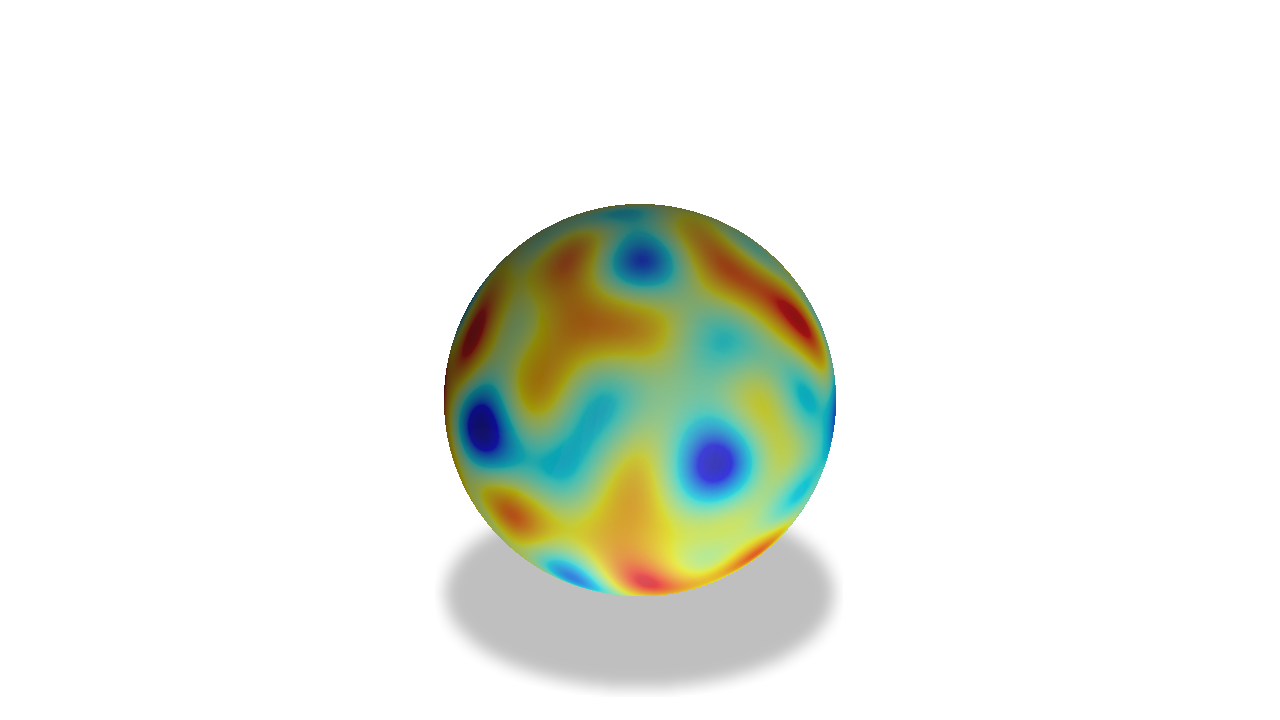
\includegraphics[width=\linewidth]{Chapter5/figures/sphere.png}
% %   \caption{Manifolds}
%   \label{fig:1}
% \end{subfigure}\hfil % <-- added
% \begin{subfigure}{0.25\textwidth}
%   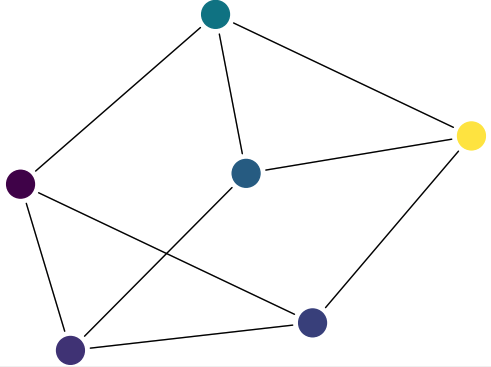
\includegraphics[width=\linewidth]{Chapter5/figures/graph.png}
% %   \caption{Graphs}
%   \label{fig:2}
% \end{subfigure}\hfil % <-- added
% \begin{subfigure}{0.25\textwidth}
%   \includegraphics[width=\linewidth]{Chapter5/figures/BunnyWire.png}
% %   \caption{Meshes}
%   \label{fig:3}
% \end{subfigure}

% \medskip
% \begin{subfigure}{0.25\textwidth}
%   \includegraphics[width=\linewidth]{Chapter5/figures/cosmos.png}
% %   \caption{Cosmos}
%   \label{fig:4}
% \end{subfigure}\hfil % <-- added
% \begin{subfigure}{0.25\textwidth}
%   \includegraphics[width=\linewidth]{Chapter5/figures/social_network.png}
% %   \caption{image5}
%   \label{fig:5}
% \end{subfigure}\hfil % <-- added
% \begin{subfigure}{0.25\textwidth}
%   \includegraphics[width=\linewidth]{Chapter5/figures/mesh_engine.png}
% %   \caption{image6}
%   \label{fig:6}
% \end{subfigure}
% \caption{Domains (top) and applications (bottom)}
% \label{fig:images}
% \end{figure}

\paragraph{Collaborators}
\begin{enumerate}
    \item Alex Terenin (Imperial College London)
    \item Willie Neiswanger (Stanford University)
\end{enumerate}


\section{Projects in Progress}
\begin{enumerate}
    \item ``Pay Attention to Deep Gaussian Processes''\\
    Transformer Layer Gaussian Processes using an explicit feature representation of the attention operation.
    \begin{equation*}
        \exp(\vx^\top \vy) = \Phi^\top(\vx) \Phi(\vy)
    \end{equation*}
    \item A Unifying Theory for Interdomain Gaussian Processes.
    \item VISH-PI: Probabilistic Integration with Variational Inducing Spherical Harmonics.
\end{enumerate}


% \section{Understanding Deep Learning through Gaussian Processes}

% \begin{enumerate}
%     \item 
% \end{enumerate}
